\chapter{System Overview}
\label{ch:overview}

\section{Application Overview}
The application is a single-page application (SPA) built with React and
Vite, communicating with a PHP backend through a JSON HTTP API. The browser
never performs a full page reload while navigating between the game, the
dashboard, the leaderboard, and the history page; instead, React Router
switches between page components while shared state (authentication and
theme) is provided through React Context.

\section{Target Users}
The system supports a single user role:
\begin{itemize}[nosep]
    \item \textbf{Registered Player} -- creates an account, plays timed
    Minesweeper games at one of two difficulties, and can view a personal
    dashboard of statistics, a full history of past games, and a global
    leaderboard of top scores across all players.
\end{itemize}
There is no administrator or moderator role; every authenticated user has
identical privileges over their own data.

\section{System Workflow}
At a high level, a player's session follows the flow shown in
Figure~\ref{fig:user-flow}: the player registers or logs in, is taken to a
dashboard, starts a game at a chosen difficulty, plays until the game ends
(by mine or timeout), and the result is automatically submitted to the
backend and reflected in the player's history, statistics, and the global
leaderboard.

\begin{figure}[h]
    \centering
    \begin{tikzpicture}[node distance=1.6cm, every node/.style={font=\small}]
        \tikzstyle{block} = [rectangle, rounded corners, draw=black, thick,
            fill=orange!15, text width=2.6cm, align=center, minimum height=1cm]
        \tikzstyle{arrow} = [-{Latex[length=2mm]}, thick]

        \node (login) [block] {Register / Login};
        \node (dash) [block, right=of login] {Dashboard};
        \node (play) [block, right=of dash] {Select Difficulty \& Play};
        \node (end) [block, right=of play] {Game Ends \\ (mine or timeout)};
        \node (save) [block, below=of end] {Score Recomputed \& Saved (Backend)};
        \node (views) [block, left=of save] {History / Stats / Leaderboard Updated};

        \draw [arrow] (login) -- (dash);
        \draw [arrow] (dash) -- (play);
        \draw [arrow] (play) -- (end);
        \draw [arrow] (end) -- (save);
        \draw [arrow] (save) -- (views);
    \end{tikzpicture}
    \caption{High-level player workflow.}
    \label{fig:user-flow}
\end{figure}

\section{Main Modules}
The application is organized into the following functional areas, described
in detail in later chapters:
\begin{itemize}[nosep]
    \item \textbf{Authentication Module} -- registration, login, and logout
    endpoints backed by PHP sessions (\texttt{register.php},
    \texttt{login.php}, \texttt{logout.php}).
    \item \textbf{Game Engine Module} -- the pure functional board logic in
    \texttt{minesweeper.js} and the stateful \texttt{useMinesweeper} hook
    that drives it.
    \item \textbf{Score Persistence Module} -- the \texttt{save-score.php}
    endpoint, which validates and recomputes a submitted result before
    writing it to the \texttt{game\_results} table.
    \item \textbf{Statistics and History Module} -- the
    \texttt{leaderboard.php}, \texttt{history.php}, and \texttt{stats.php}
    endpoints and their corresponding React pages.
\end{itemize}

\section{Screenshots}
Figures~\ref{fig:login-page} and~\ref{fig:register-page} show the
authentication screens; Figure~\ref{fig:dashboard-page} shows the
authenticated dashboard.

\begin{figure}[h]
    \centering
    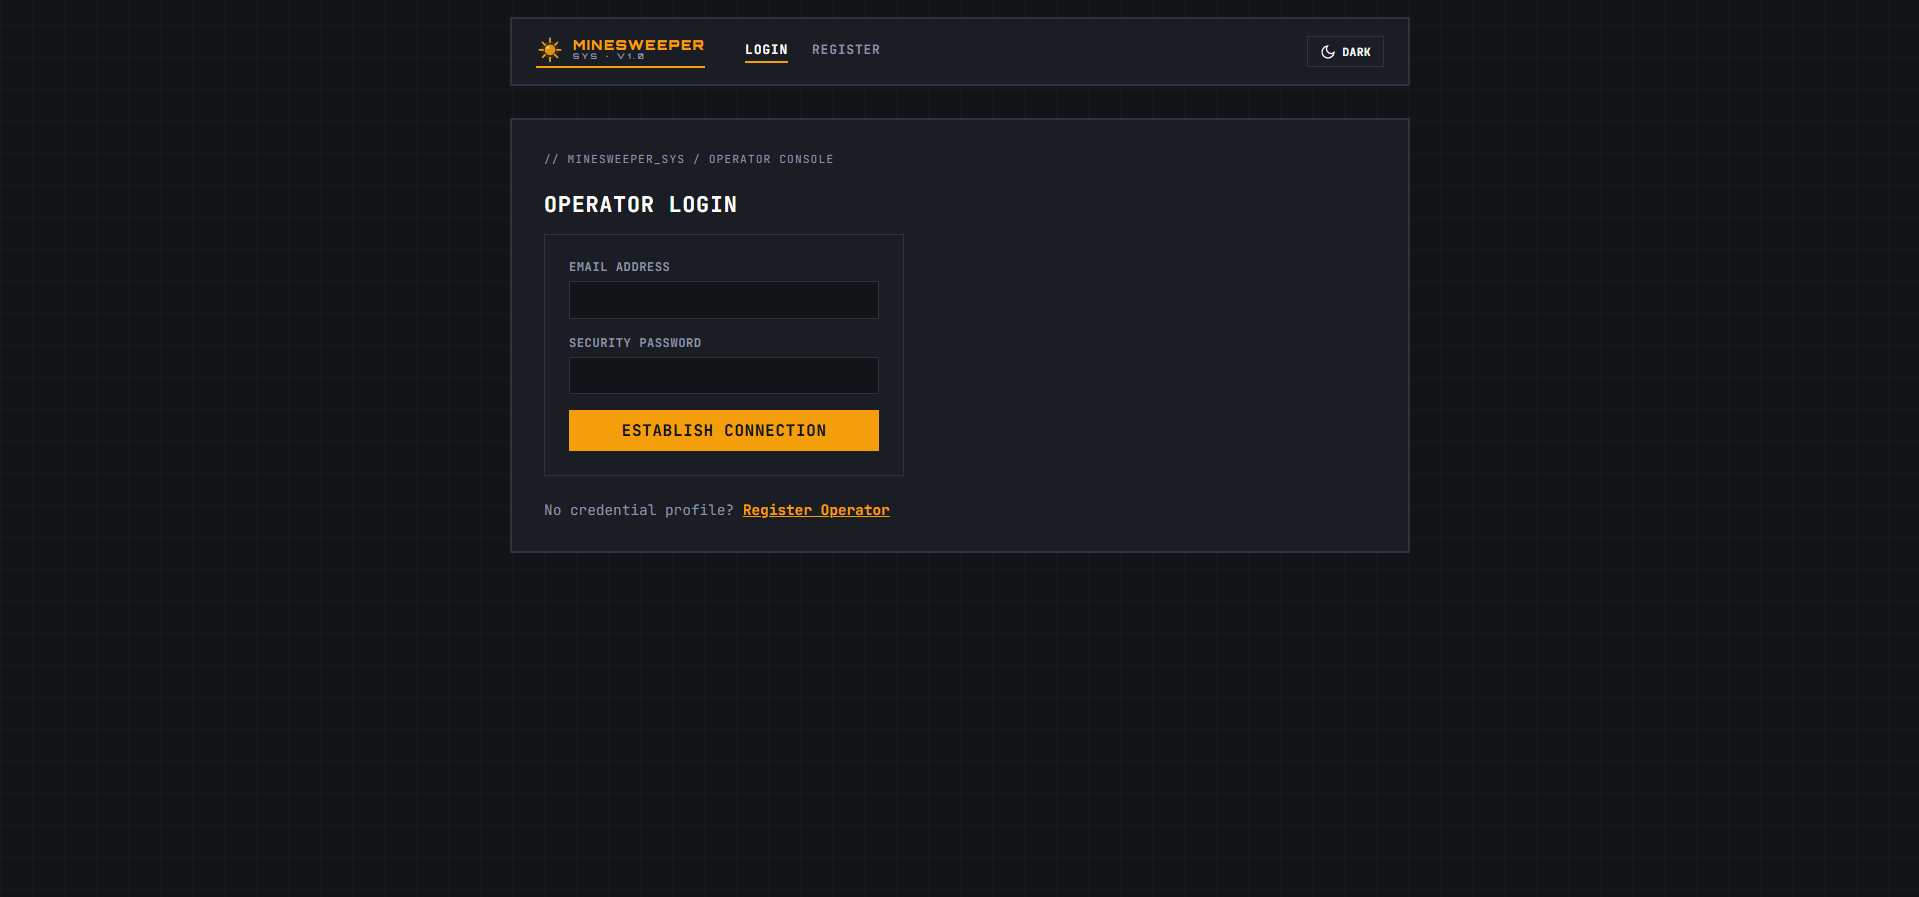
\includegraphics[width=0.8\textwidth]{figures/fig_login.png}
    \caption{Operator login page.}
    \label{fig:login-page}
\end{figure}

\begin{figure}[h]
    \centering
    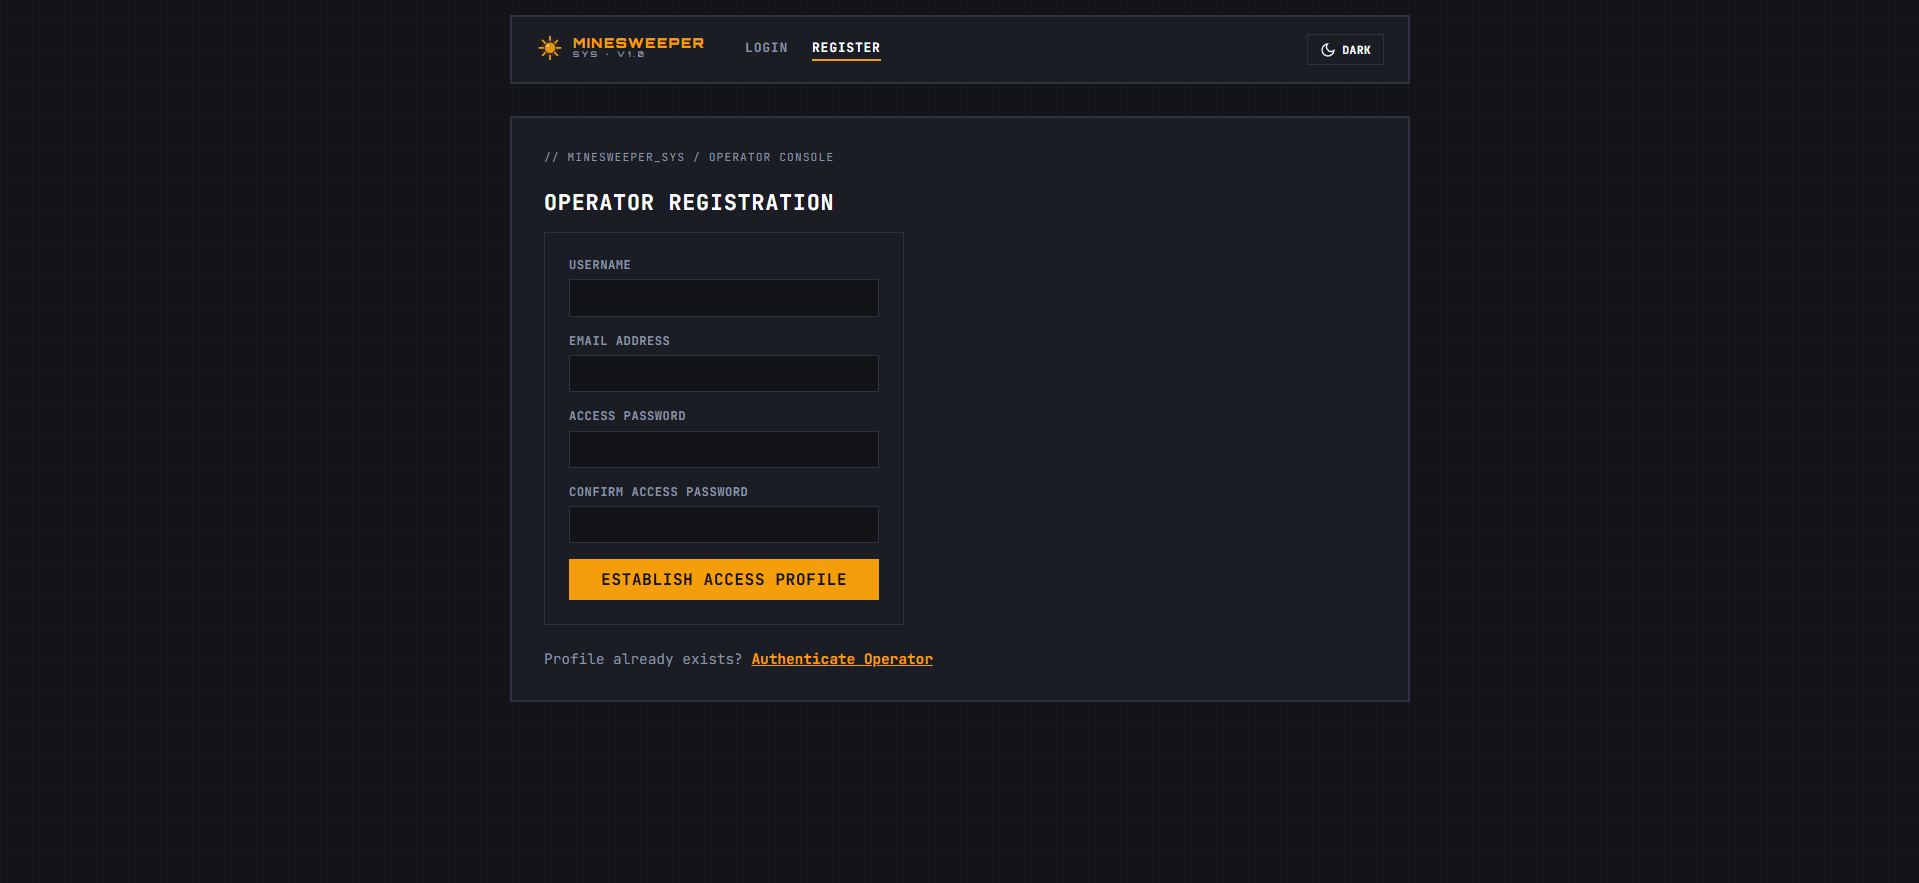
\includegraphics[width=0.8\textwidth]{figures/fig_register.png}
    \caption{Operator registration page.}
    \label{fig:register-page}
\end{figure}

\begin{figure}[h]
    \centering
    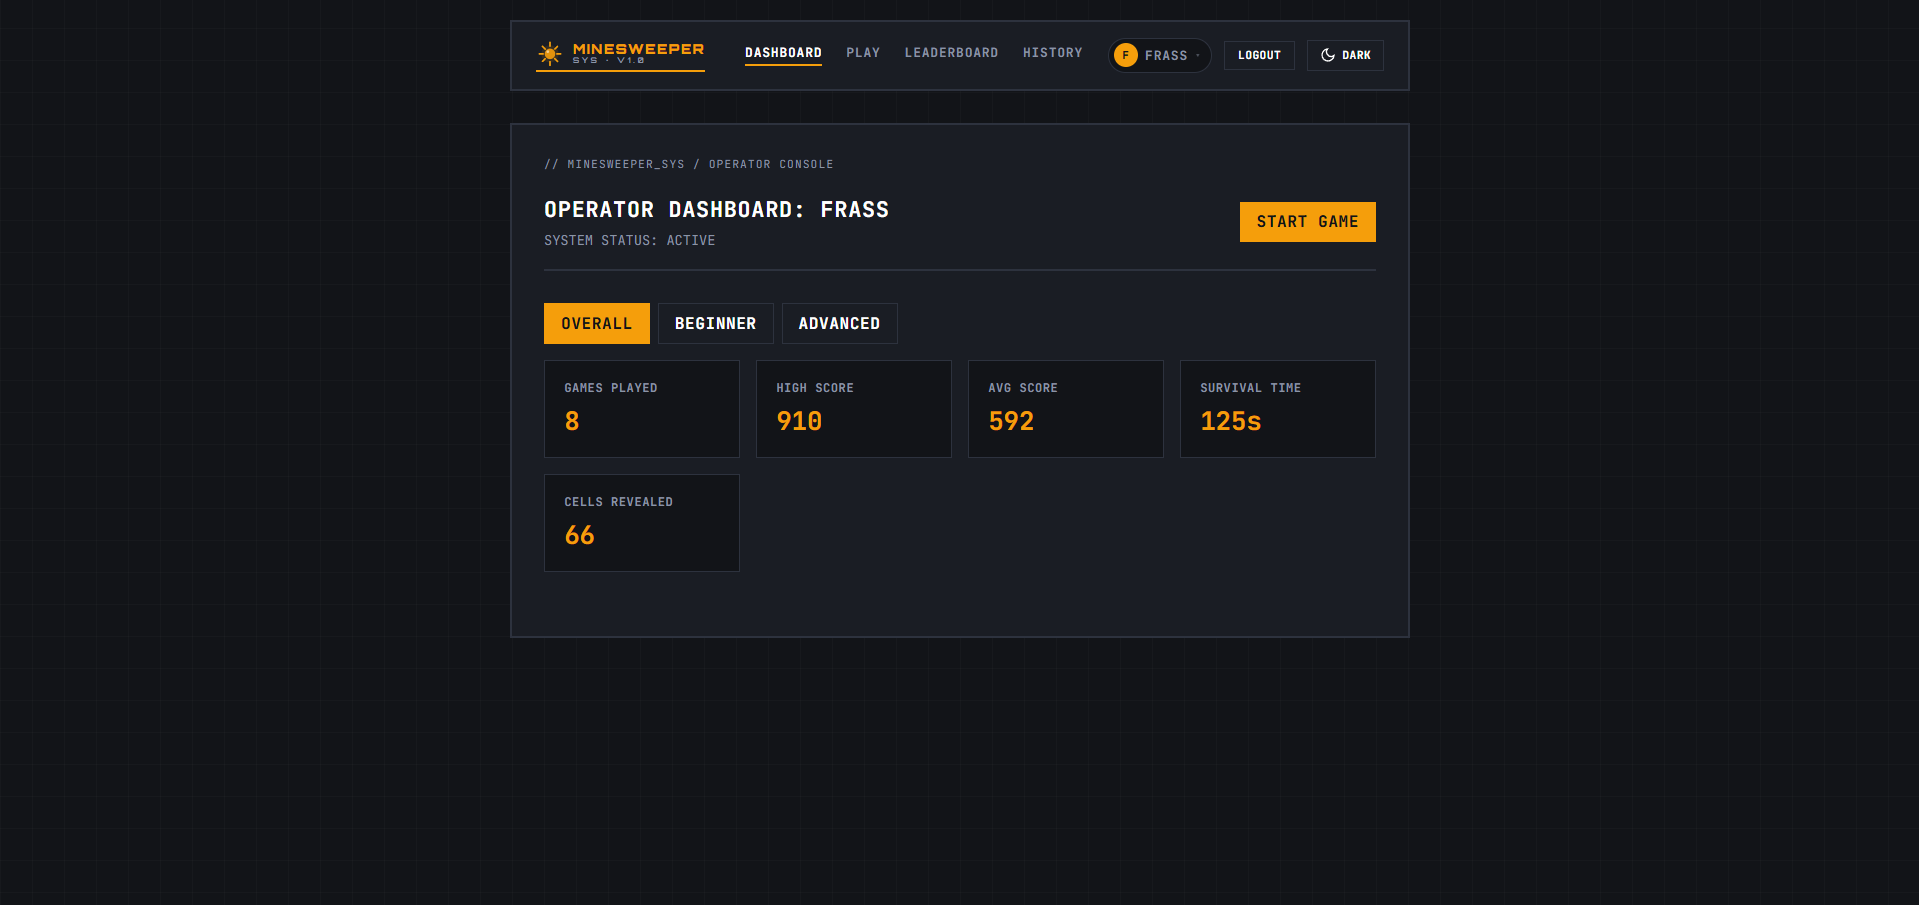
\includegraphics[width=0.8\textwidth]{figures/fig_dashboard_dark.png}
    \caption{Player dashboard showing combat statistics and quick-access links.}
    \label{fig:dashboard-page}
\end{figure}
